\chapter{Grundlagen}\label{ch:grundlagen}

In diesem Kapitel werden Grundlagen zu den relevanten Begriffen der Domäne erläutert. Zunächst wird hierzu die Online-Plattform INLOOP beschrieben. Danach werden die Konzepte, Ziele und Probleme hinter Gamification und Codequalitätsanalyse diskutiert und schließlich zusammengefasst.

\section{INLOOP}\label{sec:inloop}

INLOOP ist eine Webanwendung, die an der Technischen Universität Dresden entwickelt wurde. Die Webanwendung wird im Rahmen der Lehrveranstaltung Softwaretechnologie genutzt, um deren didaktisches Konzept durch ein fakultatives Angebot von Online-Programmieraufgaben zu erweitern. Das didaktische Konzept beinhaltet als Lernziele dabei unter anderem, dass die Studierenden anhand der Programmiersprache Java objektorientierte Konzepte (Entwurfsmuster, Klassenbibliotheken, UML-Modelle) implementieren und diese Implementation einer Software-Qualitätssicherung unterziehen können \cite{asmann_modulbeschreibung_2010}. In INLOOP können Programmieraufgaben veröffentlicht und in verschiedene Kategorien unterteilt werden. Die Kategorien (Basic, Lesson, Exam) sind hierbei nach steigender Komplexität und Schwierigkeit geordnet. Die in diese Kategorien eingegliederten Programmieraufgaben bestehen aus einer textuellen Beschreibung. In der textuellen Beschreibung der meisten Aufgaben sind außerdem Diagramme integriert, welche zum Beispiel die Klassenstruktur der zu implementierenden Software repräsentieren (in Form von UML-Analyse/Entwurf-Klassendiagrammen) oder die Reihenfolge und Art von zwischen Komponenten der Software ausgetauschten Informationen (in Form von UML-Sequenzdiagrammen oder UML-Zustandsdiagrammen) aufzeigen. Aufgaben können von Nutzern der Plattform, entweder in einer eigenen Entwicklungsumgebung oder in einem integrierten Online-Editor, von zuhause bearbeitet werden. Die eingereichten Lösungen werden in der Plattform auf funktionelle Korrektheit geprüft und hierdurch automatisiert ausgewertet. Zum Schluss eines jeden Bearbeitungsprozesses wird ein direktes Feedback zur funktionellen Korrektheit der Teilkomponenten der eingereichten Lösung präsentiert. Besteht eine Lösung nicht alle funktionellen Tests, so wird sie als \enquote{nicht bestanden} gewertet. Als logische Konsequenz ist eine Lösung auch nur dann \enquote{bestanden}, wenn alle funktionellen Tests erfolgreich waren. INLOOP gliedert sich mit diesem didaktisch orientierten Grundkonzept in die so genannten E-Learning-Systeme ein und hat somit den primären Zweck, Lehrinhalte zu vermitteln und den Nutzern der Plattform beim Erlernen neuer Inhalte zu helfen. Da die Inhalte darüber hinaus auch abgefragt und bewertet werden können, repräsentiert INLOOP gleichzeitig ein so genanntes E-Assessment-System \cite{handke_e-learning_2012}. \Cref{fig:assessment} zeigt den im Fokus stehenden Lernprozess als Iterationszyklus, zu dessen Schluss das durch die automatisierte Beurteilung in INLOOP realisierte summative Assessment steht.

\begin{figure}[H]
\centering
\includegraphics[width=\linewidth, bb=0 0 462 132]{assessment.pdf}
\caption{Varianten des Assessments anhand des iterativen Lernzyklus. Angelehnt an \cite[S. 44]{handke_e-learning_2012} und basierend auf \cite[S. 41]{crisp_e-assessment_2007}.}\label{fig:assessment}
\end{figure}

\noindent Die Aufgaben in INLOOP werden über das laufende Semester für die Studierenden in zeitlich aufeinanderfolgenden Abschnitten über ein eigenes Versionsmanagement freigegeben, sodass zu Anfang des Semesters noch keine der schwierigeren und komplexeren Exam-Aufgaben verfügbar sind. Die Studierenden können sich somit zu Beginn des Semesters auf die verhältnismäßig einfacheren und grundlegenderen Aufgaben konzentrieren. Hierbei ist zu beachten, dass Aufgaben als befristet definiert werden können, also nur bis zum Verfall einer bestimmten Deadline abgegeben werden können. Zur Motivation der Studierenden, das fakultative Angebot zu nutzen, werden als Anreiz Bonuspunkte für die Klausur verliehen. Die genauen Details und Rahmenbedingungen können die Studierenden dabei auf INLOOP einsehen\footnote{Bonuspoint rules. \url{https://inloop.inf.tu-dresden.de/about/bonuspoint-rules/} (Abgerufen am 13.6.2020)}. Bonuspunkte werden hierbei nur vergeben, wenn die in Frage kommende Lösung nicht plagiiert wurde. Für die Plagiatsprüfung der Java-basierten Lösungen wird JPlag\footnote{JPlag. \url{https://jplag.ipd.kit.edu/} (Abgerufen am 13.6.2020)} verwendet. Mit der Einführung von INLOOP und mithilfe der Bonuspunkte als Motivator konnte beobachtet werden, dass sich hierdurch vermehrt Studierende an den bereitgestellten Programmieraufgaben probierten und schließlich im Vergleich besser in der Abschlussprüfung der Lehrveranstaltung abschnitten \cite{morgenstern_continuous_2018}.

\section{Gamification}

Analog zu den beschriebenen Bonuspunkten etablierte sich in den vergangenen Jahren ein als \enquote{Gamification} bezeichnetes Prinzip als weitere Möglichkeit, die Motivation von Nutzern zu steigern. Durch den Einsatz dieses Prinzips konnte in verschiedenen Studien nachgewiesen werden, dass hierdurch die Leistungen der Nutzer innerhalb des jeweiligen Kontextes signifikant gesteigert werden konnten \cite{mekler_points_2013}\cite{sheth_increasing_2012}\cite{akpolat_enhancing_2014}. Einige universitäre Online-Plattformen, beispielsweise das Auditorium-Forum der TU Dresden\footnote{Auditorium. \url{https://auditorium.inf.tu-dresden.de/} (Abgerufen am 14.9.2020)} oder die OUTPUT.DD-App\footnote{OUTPUT.DD-App. \url{https://play.google.com/store/apps/details?id=de.tud.android.outputdd&hl=de} (Abgerufen am 14.9.2020)}, nutzen Gamification bereits zur Motivation der Nutzer. Daher wird nach der begrifflichen Einordnung in dieser Sektion betrachtet, wie die motivierende Wirkung anhand des Einsatzes bestimmter Elemente interpretiert werden kann und auf welchen psychologischen Grundbedürfnissen dies fußt. Anschließend werden Gamification-Frameworks anhand des nutzerorientierten Octalysis-Frameworks betrachtet, mithilfe derer eine Gamification aus verschiedenen Perspektiven umgesetzt werden kann.

\subsection{Begriffliche Einordnung}\label{sec:gamification-begriff}

\begin{defs}
Gamification ist die Anwendung von aus Spielen bekannten charakteristischen Gestaltungselementen auf nicht spielbezogene Kontexte \cite[sinngemäß übersetzt]{deterding_game_2011}.
\end{defs}

\noindent Deterding et al. beschreiben die Ursprünge des Begriffs in der Industrie der digitalen Medien um das Jahr 2008, wobei sich der Begriff Gamification erst im Jahr 2010 weitläufig gegenüber koexistierenden Synonymen wie \enquote{Funware} oder \enquote{Applied Gaming} etabliert habe. Die Arbeit der Autoren schaffte eine kommunikative Grundlage, indem sie die domänenspezifischen Begriffe durch differenzierte Betrachtung taxonomisch einordnete \cite{deterding_game_2011}. Die Autoren grenzen den Begriff Gamification hierbei von so genannten \enquote{Serious Games} ab. Sie beschreiben Serious Games als Spiele, die einen ernsten Verwendungszweck haben, meist die Vermittlung von Lerninhalten. Im Unterschied hierzu sei Gamification interpretierbar als eine Verwendung von aus Spielen bekannten charakteristischen Gestaltungselementen auf \textit{nicht spielbezogene} Kontexte. Gleichzeitig differenzieren die Autoren zwischen einem \enquote{Playful Design} und einem \enquote{Gameful Design}. Dem Playful Design liegt eine \enquote{Playfulness} zugrunde, die eine Denkweise beschreibt, bei der spielerische Tätigkeiten ohne Ernsthaftigkeit, klarem Ziel oder echten Konsequenzen ausgeführt werden \cite{lucero_playful_2014}. Gameful Design wiederum als Grundlage der Gamification sei komplementär zum Playful Design durch bestimmte Regeln, Handlungsweisen, Akteure, Ziele und Ergebnisse (\enquote{Gaming}) charakterisiert, wobei diese durch eine \enquote{Gameful Experience} kombiniert und erfahrbar gemacht werden.

\subsection{Gamification-Elemente}\label{sec:gamification-elemente}

Eine wichtige Grundlage für das erfahrbar Machen einer \enquote{Gameful Experience} besteht in der Verwendung von so genannten Gamification-Elementen.

\begin{defs}
Gamification-Elemente sind charakteristische Gestaltungselemente der Gamification, welche in den meisten (jedoch nicht zwangsweise allen) Spielen gefunden und mit diesen assoziiert werden können und dort eine signifikante Rolle im Spielablauf einnehmen \cite[Sinngemäß übersetzt]{deterding_game_2011}.
\end{defs}

\noindent Im Folgenden werden typische Gamification-Elemente beschrieben \cite[angelehnt an die Kategorisierung von Sailer et al.]{sailer_how_2017}.

\paragraph{Punkte} repräsentieren den Fortschritt und Erfolg des Spielers, als quantitative Grundlage für verschiedene weitere Gamification-Elemente, wobei als Spieler die Nutzer der Anwendung im Rahmen der Gamification gemeint sind. Schließt ein Spieler eine Handlung innerhalb der Anwendung mit Erfolg ab, erhält dieser dafür eine Punktzahl. Die jeweils erreichten Punktzahlen werden in der Regel in einem Gesamtpunktestand aggregiert. Punkte können in verschiedenen Formen und Verwendungen auftreten, z.B. in Form von Erfahrungspunkten als Grundlage für die Bestimmung einer Erfahrungsstufe (Level), oder in Form einer Währung, welche für bestimmte Gegenleistungen innerhalb der Anwendung eingetauscht werden kann.

\paragraph{Errungenschaften} sind visuelle Repräsentationen des Erreichens von im Voraus festgesetzten Zielen durch einen Spieler. Sie kommen häufig in der Form von Trophäen oder Badges vor und können vom Spieler durch die Erfüllung von bestimmten Zielen erhalten werden. Meist werden diese Errungenschaften danach für andere Spieler sichtbar auf dem jeweiligen Profil präsentiert.

\paragraph{Ranglisten} führen Spieler sortiert nach ihrer Punktzahl oder nach einer ähnlichen Metrik auf, wie zum Beispiel die Dauer für das Erledigen einer Aufgabe. Somit hat jeder Spieler die Möglichkeit, sich bezüglich der jeweiligen Metrik mit anderen Spielern zu vergleichen.

\paragraph{Leistungsgraphen} zeigen dem Spieler, wie sich seine Leistung bei einer Aufgabe im Laufe der Zeit oder im Vergleich zu einem vorigen Durchlauf verändert. Die visuelle Darstellung wird realisiert über die Darstellung der Leistung in Relation zur Zeit durch einen Graphen. Im Unterschied zu Ranglisten wird hierbei also der Spieler mit sich selbst verglichen und nicht mit anderen Spielern.

\paragraph{Narrative} werden in den bestehenden Anwendungskontext eingebunden und beziehen sich im Vergleich zu den oben genannten Gamification-Elementen nicht auf die Leistung des Spielers. Das Grundkonzept hierbei ist, die im Rahmen der Anwendung zu lösenden Aufgaben oder auszuführenden Tätigkeiten in eine Geschichte zu integrieren. Dies kann beispielsweise über eine narrative Rahmenhandlung mit eigenen Charakteren geschehen.

\paragraph{Avatare} zeigen die Spieler als Spielfigur innerhalb der Anwendung. In der Regel ist es dem Spieler möglich, den eigenen Avatar zu erstellen und zu modifizieren. Dies kann zum Beispiel in Form von simplen zweidimensionalen Grafiken geschehen.

\paragraph{Teammitglieder} können echte oder durch den Computer gesteuerte Mitspieler sein, die zusammen mit dem Spieler in einer Gruppe bestimmte Aufgaben lösen.

\subsection{Gamification als Motivator}\label{sec:gamification-motivator}

Sailer et al. analysierten die beobachtete Leistungssteigerung bei der Anwendung von Gamification als Resultat aus der motivierenden Wirkung \cite[p. 4,5]{sailer_how_2017} auf die Nutzer. Die motivierende Wirkung sei ein Resultat daraus, dass die Einführung der charakteristischen Gestaltungselemente auf die Erfüllung von psychologischen Grundbedürfnissen abzielte, konkreter:

\begin{itemize}
\item das \textbf{Bedürfnis nach Kompetenz}\label{gamification:need-for-competence}, erfüllbar durch ein Gefühl der Effizienz und des Erfolges bei der Interaktion,
\item das \textbf{Bedürfnis nach Freiheit bei der Wahl einer Aufgabe}\label{gamification:need-for-autonomy-of-decision-freedom},
\item das \textbf{Bedürfnis nach Freiheit bei der Einschätzung der Sinnhaftigkeit einer Aufgabe}\label{gamification:need-for-autonomy-of-task-meaningfulness} und der damit einhergehenden Freiheit, zu entscheiden, in welchem Maße die Aufgabe zu erfüllen ist sowie
\item das \textbf{Bedürfnis nach sozialer Verbundenheit}\label{gamification:need-for-autonomy-of-social-relatedness}.
\end{itemize}

\noindent Sailer et al. diskutierten die psychologischen Grundlagen der Gamification anhand der Wirkung der typischen Gamification-Elemente. Sie beschreiben, mithilfe von Punkten könne dem Spieler ein belohnendes direktes Feedback für die von ihm getätigten Aktionen übermittelt werden. Da hiermit bereits einzelne Aktionen oder Teile von diesen belohnt werden, bezeichnen Sailer et al. dies als granulares Feedback. Weiterhin erklären sie, Punkte könnten dem Spieler seinen eigenen Fortschritt visualisieren und damit \hyperref[gamification:need-for-competence]{das Bedürfnis nach Kompetenz} erfüllen. Durch Errungenschaften in Form von Badges würde dem Nutzer weiterhin die Möglichkeit gegeben werden, bestimmte Ziele zu erreichen und dies jeweils nach außen als \enquote{virtuelles Statussymbol} zeigen zu können, führen die Autoren weiterhin auf. Verweisend auf Wang und Sun \cite{wang_game_2012} beschreiben die Autoren, dass gleichzeitig Spieler durch den Einsatz von Badges zur Erfüllung bestimmter Aufgaben motiviert werden könnten. Da Errungenschaften nach einer Reihe von bestimmten Handlungen vergeben werden, kategorisieren Sailer et al. anhand von Badges dies auch als kumulatives Feedback. Ähnlich zu Punkten bedienten Badges auch das \hyperref[gamification:need-for-competence]{Bedürfnis nach Kompetenz}. Zum Gamification-Element Ranglisten fassen Sailer et al. zusammen, dass mithilfe dessen Spieler motiviert werden könnten, andere Mitspieler zu übertreffen. Ranglisten wirkten als soziales Druckmittel, schlussfolgern die Autoren. Es habe sich jedoch gezeigt, dass Ranglisten auch eine demotivierende Wirkung haben können, wenn sich beispielsweise der jeweilige Nutzer im unteren Bereich der Ranglisten wiederfindet. Sie empfehlen daher, Ranglisten so zu gestalten, dass die im Vergleich zum Spieler in der Rangliste gezeigten konkurrierenden Spieler eine ähnliche Punktzahl wie dieser haben. Sailer et al. ordnen Ranglisten, analog zu Punkten, der Erfüllung \hyperref[gamification:need-for-competence]{des Bedürfnisses nach Kompetenz} in Form von einem kumulativen Feedback zu. Weiterhin diskutieren Sailer et al. zu dem Gamification-Element Leistungsgraphen, dass sich durch die Präsentation der Leistung über eine feste Zeitspanne ein Bedürfnis für den Spieler bilde, sich selbst zu verbessern. Leistungsgraphen zielten somit auch \hyperref[gamification:need-for-competence]{auf das Bedürfnis nach Kompetenz} ab, indem sie dem Spieler ein nachhaltiges Feedback gäben. Als Ziel von sinnvollen Narrativen nennen die Autoren, dass Aufgaben für den Nutzer gehaltvoller und weniger langweilig wirken sollen. Durch die gesteigerte Attraktivität der jeweiligen Aufgabe ziele dieses Gamification-Element ab auf das \hyperref[gamification:need-for-autonomy-of-task-meaningfulness]{Bedürfnis des Spielers nach Freiheit, eine Aufgabe zu bearbeiten und dabei die Sinnhaftigkeit dieser einzuschätzen}. Gleichzeitig könnten Narrative gezielt als Analogie zu Prozessen aus der \enquote{echten} Welt gewählt werden. Sailer et al. erläutern Avatare als Möglichkeit, durch deren Wahl und Erstellung freie Entscheidungen innerhalb des Kontextes getroffen werden können. Sie richteten sich somit an die Erfüllung des \hyperref[gamification:need-for-autonomy-of-decision-freedom]{Bedürfnisses der Entscheidungsfreiheit}. Zum von Sailer et al. kategorisierten Gamification-Element der Teammitglieder beschreiben die Autoren schließlich, durch die Bearbeitung eines gemeinsamen Ziels im Team würde hierbei das \hyperref[gamification:need-for-autonomy-of-social-relatedness]{Bedürfnis nach sozialer Verbundenheit} erfüllt.

\subsection{Frameworks}\label{sec:gamification-frameworks}

Gamification-Ansätze können scheitern, wenn deren Grundlage eine ungeeignete Auswahl oder eine ungeeignete Kombination von Gamification-Elementen ist oder der zugrundeliegende Game-Design Prozess nicht stringent genug durchgeführt wird, beschreiben Mora et al. und analysieren daher eine Reihe von Gamification-Frameworks, welche den Gestaltungsprozess strukturieren sollen \cite{mora_literature_2015}. Im Folgenden wird das Gamification-Framework \enquote{Octalysis} als Beispiel betrachtet. Der Gamification-Experte Yu-kai Chou illustriert die Notwendigkeit eines guten Game-Designs als Grundgerüst, welches einzelne Gamification-Elemente zusammenhält. Er karikiert dies anhand eines \enquote{schlechten} Game-Designers, der bestimmte Elemente und Spielmechaniken allein anhand ihrer Popularität in anderen Anwendungen zusammenstellt, ohne auf ein gutes Game-Design zu achten \cite[S. 21ff]{chou_actionable_2019}. Ein \enquote{guter} Game-Designer würde sich nach Chous Interpretation zu Beginn fragen, welche Emotionen er beim Nutzer auslösen möchte und auf Grundlage dessen bestimmte Elemente und Spielmechaniken auswählen, mit denen diese Emotionen erzeugt werden könnten. In seinem \enquote{Octalysis} Gamification Framework beschreibt Chou einen Gamification-Ansatz, bei dem die gewählten Methoden konzentrisch auf die Bedürfnisse und Ziele des Nutzers hinwirken. Chou analysierte hierfür verschiedene Spiele und warum einige dieser Spiele (teilweise gegenüber fast äquivalenten Kopien dieser) erfolgreich waren. Er fasst acht Kernantriebe einer Gamification zusammen:

\begin{enumerate}
\item \textbf{Epic Meaning and Calling:} Die erzählerische Bedeutsamkeit der dargestellten Inhalte und \enquote{Berufung} des Spielers, indem dieser für die Lösung der Aufgabe auserwählt wird.
\item \textbf{Development and Accomplishment:} Die Möglichkeit, fortzuschreiten und dabei über Herausforderungen Errungenschaften zu erzielen.
\item \textbf{Empowering of Creativity and Feedback:} Die Möglichkeit, dass Spieler zur Lösung von Aufgaben kreativ sein können und hierbei Ergebnisse dessen beobachten können.
\item \textbf{Ownership and Possession:} Die Möglichkeit des Besitztums und der Akquise von weiterem Besitz.
\item \textbf{Social Influence and Relatedness:} Die Förderung der sozialen Interaktion.
\item \textbf{Scarcity and Impatience:} Die Reduktion der Verfügbarkeit von bestimmten Ressourcen oder die zeitliche Beschränkung von bestimmten Aktivitäten.
\item \textbf{Unpredictability and Curiosity:} Die Möglichkeit, Dinge zu entdecken oder überrascht zu werden.
\item \textbf{Loss and Avoidance:} Die Gefahr, etwas zu verlieren oder zu verpassen.
\end{enumerate}

\begin{figure}[H]
\centering
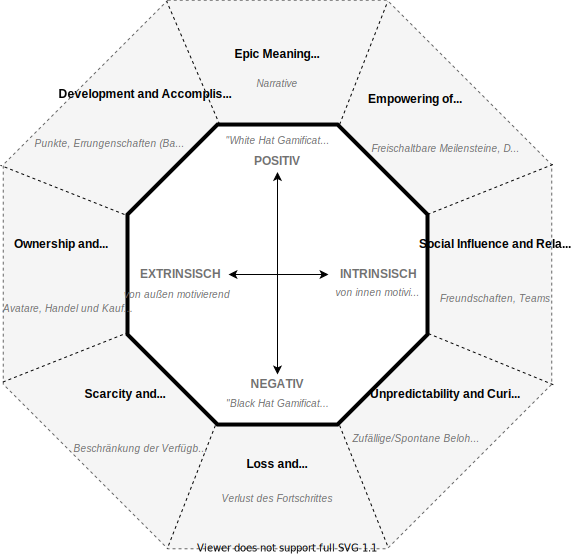
\includegraphics[width=0.75\linewidth, bb=0 0 408 402]{octalysis.pdf}
\caption{Die von Yu-kai Chou entwickelte Gamification-Taxonomie \enquote{Octalysis} als Oktagon mit beispielhaften Gamification-Elementen. Mit freundlicher Genehmigung \cite{chou_actionable_2019}.}\label{fig:octalysis}
\end{figure}

\noindent Weiterhin ordnet Chou diesen Teilzielen die jeweiligen Gamification-Elemente zu. So seien die weit verbreiteten Gamification-Elemente Punkte, Ranglisten und Errungenschaften (bspw. in Form von Badges) zuzuordnen in die Kategorie \enquote{Development and Accomplishment}. Die in \Cref{fig:octalysis} gezeigte Anordnung der acht Teilziele teilt Chou nochmals horizontal und vertikal. Die links in der Abbildung gezeigten Ziele zielten auf die durch äußere Reize hervorrufbare (extrinsische) Motivation des Nutzers ab, während die rechts gezeigten Ziele die von dem Nutzer selbst stammende (intrinsische) Motivation unterstützten. Außerdem seien die weiter oben angebrachten Ziele positiver als die weiter unten gezeigten Ziele, wie zum Beispiel \enquote{Loss and Avoidance}. Diese Teilung illustriert Chou als \enquote{White Hat Gamification} und \enquote{Black Hat Gamification}, was eine Analogie zum legalen White Hat Hacking und zum illegalen Black Hat Hacking darstellt. Eine nach diesen Zielen orientierte Gamification bezeichnet Chou als \enquote{Level 1 Octalysis}. Unter \enquote{Level 2 Octalysis} beschreibt er eine Gamification, welche die genannten Ziele der jeweiligen Phase des Spielers anpasst, wobei der Spieler das Spiel zunächst entdeckt, danach dessen Regeln erlernt und Ziele erreichen möchte und schließlich nach erreichen aller Ziele nach weiteren Motivationen sucht. Zusätzlich ließe sich hieran nach Chou die \enquote{Level 3 Octalysis} anschließen, die diese Faktorisierung der Spielphasen noch zusätzlich um eine Faktorisierung der Spielertypen erweitert.

\section{Softwarequalität}

In der folgenden Sektion werden die Grundlagen zum komplexen Begriff der Softwarequalität aufgeschlüsselt, um die Codequalität hierin schließlich systematisch einzuordnen und Möglichkeiten aufzuzeigen, diese in einem komplexen Softwaresystem abzubilden. Hierfür werden zunächst unterschiedliche Perspektiven erläutert, aus denen die Qualität einer Software betrachtet werden kann. Nachfolgend wird die Codequalität in eine dieser Perspektiven eingeordnet, um die Konsequenzen aus einer guten oder schlechten Codequalität für die Gesamtqualität der Software ableiten zu können und die Relevanz der Codequalität als zentrale Qualitätskomponente in der Gesamtqualität von Software zu zeigen. Außerdem wird beschrieben, wie deren Analyse über Codequalitätsmetriken funktionieren kann. Als zentraler Prozess in der Verbesserung von Softwarequalität wird schließlich der Vorgang der Refaktorisierung erklärt und mit dem Begriff der technischen Schulden in Verbindung gebracht sowie aufgezeigt, inwiefern dies automatisierbar ist.

\subsection{Komponenten und Faktoren}

Die Norm ISO/IEC 9126:2001 \cite{technical_committee_isoiec_jtc_1sc_7_software_and_systems_engineering_isoiec_2001}, aktualisiert durch ISO/IEC 25010:2011 \cite{technical_committee_isoiec_jtc_1sc_7_software_and_systems_engineering_isoiec_2011} beschreibt die Softwarequalität als komplexes Resultat aus dem Lebenszyklus von Software. Die Autoren unterteilen folgende Komponenten der Gesamtqualität von Software.

\begin{figure}[H]
\centering
\includegraphics[width=\linewidth, bb=0 0 549 277]{softwarequalitaet.pdf}
\caption{Die Kaskade der Softwarequalitätskomponenten im Lebenszyklus von Software und deren Modellindikatoren nach ISO/IEC 9126:2001 \cite{technical_committee_isoiec_jtc_1sc_7_software_and_systems_engineering_isoiec_2001}.}\label{fig:softwarequalitaet}
\end{figure}

\paragraph{Die Prozessqualität} beschreibt die Qualität der in ISO/IEC/IEEE 12207:2017 \cite{technical_committee_isoiec_jtc_1sc_7_software_and_systems_engineering_isoiecieee_2017} normierten Prozesse (Beschaffung, Lieferung, Entwicklung, Betrieb und Wartung) des Lebenszyklus einer Software.

\paragraph{Die interne und externe Qualität} wird von den Autoren beschrieben als die Charakterisierung der Software von einem internen bzw. externen Standpunkt, anhand der jeweiligen internen bzw. externen Anforderungen. \Cref{fig:softwarequalitaet} zeigt die in ISO/IEC 9126:2001 hierfür vorgeschlagenen Modellindikatoren (Funktionalität, Verlässlichkeit, Nutzbarkeit, Effizienz, Wartbarkeit und Portierbarkeit). Die interne Qualität wird hierbei über die Analyse der inneren Details der Software (Codebasis, statische und dynamische Modelle oder Dokumentation) festgestellt. Vice versa repräsentiert die externe Qualität die ohne Kenntnis dieser internen Details der Software messbare Qualität, beispielsweise durch funktionale Tests.

\paragraph{Die durch Nutzung der Software feststellbare Qualität} wird durch die Autoren definiert als die Fähigkeit der Software, die Bedürfnisse des Nutzers zu befriedigen. Sie separieren dies in die Effektivität, die Produktivität, die Sicherheit und die Zufriedenstellung bei der Nutzung.
\\

\noindent Weiterhin wird von den Autoren illustriert, dass sich die oben genannten Komponenten in dieser Reihenfolge im Lebenszyklus der Software kaskadierend gegenseitig beeinflussen (siehe \Cref{fig:softwarequalitaet}). So ist die durch Nutzung feststellbare Qualität von der externen Qualität abhängig, diese hängt wiederum von der internen Qualität ab und die interne Qualität wird schließlich beeinflusst von der Prozessqualität.

\subsection{Codequalitätsmetriken}

Die Codequalität lässt sich analog zum oben beschriebenen Schema in die interne Qualität der Software einordnen und kann nach den Kriterien der ISO/IEC 9126:2001 (Funktionalität, Zuverlässigkeit, Nutzbarkeit, Effizienz, Wartbarkeit und Wiederverwendbarkeit) \cite{technical_committee_isoiec_jtc_1sc_7_software_and_systems_engineering_isoiec_2001} beurteilt werden. Um die Konformität des Codes zu den Kriterien der internen Softwarequalität zu messen, werden typischerweise die Implementationen der einzelnen Teilkomponenten der Software anhand von bestimmten Metriken analysiert. Das grundlegende Prinzip solcher Metriken ist die Erkennung von Fehlgestaltungen verschiedener Art im Code und in dessen Dokumentation. Hierbei spielen oft der Umfang, die Komplexität und der Stil des Codes eine Rolle. Zusätzlich können Metriken eingesetzt werden, welche die Entwurfsqualität der Anwendung analysieren, zum Beispiel durch die Messung der Tiefe von Vererbungen in objektorientierten Anwendungen \cite{rosenberg_software_nodate}. Traditionelle Implementationen solcher Metriken umfassen hierzu beispielsweise die Berechnung der zyklomatischen Komplexität (McCabe-Metrik), die Bestimmung der Anzahl von Schachtelungen und Statements, die Kalkulation des Verhältnisses von Code und Kommentaren oder die Länge des Programms \cite{stamelos_code_2002}. Die Wahl, Funktionsweise und Interpretation der Metriken ist vom Kontext, zum Beispiel von der verwendeten Programmiersprache, von den Anforderungen der Software oder von der Erfahrung des Entwicklers, abhängig. Für unterschiedliche Kontexte lassen sich somit unterschiedliche Modelle zur Codequalitätsanalyse entwerfen, deren Wirkung aus der Zusammensetzung und Parametrisierung resultiert.

\subsection{Refaktorisierung}\label{sec:refaktorisierung}

Genügt die Codequalität einer Software nicht mehr den Anforderungen der Softwarequalitätsziele, so bietet sich eine Refaktorisierung an. Händler und Neumann definieren den Begriff wie folgt:

\begin{defs}
Unter Refaktorisierung versteht man die Verbesserung der internen technischen Qualität eines [Software]systems durch die Modifizierung und Restrukturierung des Quellcodes, ohne das von außen sichtbare Verhalten zu verändern. \cite{fowler_refactoring_1999}
\end{defs}

\noindent Das von außen sichtbare Verhalten ist hierbei vom Standpunkt und vom Kontext abhängig. Wird beispielsweise eine Software anhand ihrer nach außen verfügbaren Schnittstellen untersucht, so kann die interne Struktur mit Beibehaltung der äußeren Schnittstellen gänzlich verändert werden. Bei der Betrachtung einer einzelnen Komponente desselben Software-Systems, zum Beispiel anhand eines Unittests, muss die sichtbare Signatur der Komponente jedoch bei den Änderungen beibehalten werden, um nach der obigen Definition als Refaktorisierung zu gelten.

\subsection{Technische Schulden}

Um die Notwendigkeit der Refaktorisierung innerhalb einer jeweiligen Softwarekomponente zu quantifizieren, akkumulieren viele automatisierte Codeanalyseframeworks, wie zum Beispiel SonarQube\footnote{SonarQube. \url{https://www.sonarqube.org/} (Abgerufen am 14.9.2020)}, anhand einer Auswahl von Codequalitätsmetriken und anderen Metriken einen so genannten TD-Score\label{begriff:td-score}, wobei TD für \underline{T}echnical \underline{D}ebt (technische Schulden) steht. Der Score setzt sich hierbei metaphorisch zusammen aus der geschätzten Zeit, die zur Refaktorisierung der jeweiligen detektierten Fehlgestaltung notwendig wäre.

Die Art der Fehlgestaltungen kann hierbei jedoch stark variieren. Kruchten et al. unterteilen technische Schulden nochmals in Testschulden, menschliche Schulden, architekturelle Schulden, sich auf Abhängigkeiten beziehende Schulden, Dokumentationsschulden oder allumfassende amorphe Softwareschulden \cite{kruchten_technical_2012}. Kruchten et al. erklären darauf aufbauend, warum der errechnete TD-Score nicht mit den tatsächlichen technischen Schulden der Software gleichgesetzt werden sollte \cite{kruchten_technical_2012}. Die Gesamtheit von technischen Schulden sei nur schwierig durch statische Codeanalyseframeworks erfassbar, vor allem strukturelle und architekturelle Fehlgestaltungen. Zu beachten sei hierbei, dass sowohl die Codeanalyseframeworks als auch die zu analysierende Software dem technologischen Evolutions- und Alterungsprozess unterlägen.

\subsection{Codierungsrichtlinien}

Softwareentwickler können unterschiedliche Auffassungen von guter Codequalität haben. Hieraus lässt sich die Hypothese ableiten, dass Codequalitätsmetriken generell ungeeignet sind, um das Verständnis von guter Codequalität in allen Facetten zu modellieren. Pantiuchina et al. zeigten hierzu anhand eines Experimentes, dass die durch Metriken modellierbare Repräsentation von guter Codequalität nicht zwingend mit der Auffassung von Entwicklern übereinstimmt \cite{pantiuchina_improving_2018}.

Aus der Sicht des Entwicklers betrachtet, kann es, abhängig von der Zusammensetzung und Parametrisierung der Codequalitätsmetriken, zu falsch-positiven und falsch-negativen Detektionen kommen. Dies ist jedoch nicht immer von der individuellen Auffassung des Entwicklers abhängig. Händler und Neumann nennen hierzu den Fall, dass es auch bei bewusst auf eine bestimmte Art und Weise implementierten Strukturen, beispielsweise bei Entwurfsmustern, zu falsch-positiven Detektionen kommen kann. Sie begründen dies in der inhärenten Komplexität der Detektionsmechanismen \cite{haendler_serious_2019}.

\subsubsection{Konformität}

Jan Rucks befasste sich im Rahmen seiner Diplomarbeit mit der Auswahl von geeigneten Codequalitätsmetriken für das sich an die Lehrveranstaltung Softwaretechnologie zeitlich anschließende Softwarepraktikum, wo die Codequalität einiger Gruppen durch SonarQube analysiert wird \cite{rucks_erstellung_2017}. Wegen der oben genannten Schwierigkeiten ist es nicht verwunderlich, dass es Rucks nicht gelang, die Qualität einer Software (halb)-automatisch anhand einer Zusammenstellung von Qualitätsmetriken in Form einer einzigen Metrik zu messen.

Rucks evaluierte hierzu mehrere Metriken, welche bestimmte Teilaspekte der internen Softwarequalität modellieren sollen, darunter Flexibilität, Konformität, Sicherheit, Wiederverwendbarkeit, Testbarkeit, Modularität und Wartbarkeit. Rucks' Evaluation verglich dabei die Berechnungen der Metriken mit den Bewertungen der Tutoren zu der jeweiligen Gruppe sowie deren Selbsteinschätzung im Softwarepraktikum, um die Korrelation der Metriken mit der Softwarequalität zu bestimmen. Hierbei sei angemerkt, dass sowohl die Bewertungen der Tutoren als auch die Selbsteinschätzung der Gruppen gute Codequalität nicht ideal repräsentieren, was die Aussagekraft der darauf fußenden Evaluation beschränkt. Rucks destillierte aus der Evaluation dennoch als einzige signifikant mit den jeweiligen Einschätzungen der Gruppe korrelierende Metrik die der Konformität, welche sich wie folgt berechnen lässt:

\begin{equation}\label{eq:konformitaetsmetrik}
M_{CON} = 1 - \frac{N_{BLV} * 2 + N_{CRV} * 1,5 + N_{MAV} + N_{MIV} * 0,5}{N_{STA}}
\end{equation}
wobei:
\begin{conditions}
    M_{CON} & Konformitätsmetrik \\
    N_{BLV} & Anzahl der Verletzungen von \enquote{Blocker}-Regeln \\
    N_{CRV} & Anzahl der Verletzungen von \enquote{Critical}-Regeln \\
    N_{MAV} & Anzahl der Verletzungen von \enquote{Major}-Regeln \\
    N_{MIV} & Anzahl der Verletzungen von \enquote{Minor}-Regeln \\
    N_{STA} & Anzahl von Statements
\end{conditions}

\noindent Analog zu den Teilkomponenten der in \Cref{eq:konformitaetsmetrik} beschriebenen Konformitätsmetrik berechnet sich diese aus dem Verhältnis der gewichteten Anzahl an Verletzungen von Codierungsrichtlinien zu der Gesamtanzahl an Statements. Die Gewichtung stammt vom durch SonarQube kategorisierten Schweregrad der jeweiligen Verletzung der Codierungsrichtlinien, von der schwerwiegendsten Art \enquote{Blocker}, über \enquote{Major}, \enquote{Minor} bis hin zur Einstufung als \enquote{Info}. Die Beobachtung, dass die Konformität, also die Einhaltung von bestimmten Codierungsrichtlinien, die Codequalität signifikant positiv beeinflusst, beschreiben auch Dietz et al \cite{dietz_teaching_2018}. Durch die Einhaltung solcher Richtlinien würde die Lesbarkeit des Codes erhöht und hierdurch dessen Wartbarkeit verbessert. Als Konsequenz hieraus verringerten sich die Wartungskosten der Software.

% - Wang et al.: systematische Literaturreview

\subsubsection{Detektion von Code Smells}\label{sec:code-smells}

Mithilfe einer fundierten Auswahl von Codierungsrichtlinien ist es möglich, eine gegebene Software auf potenzielle Verstöße gegen diese Codierungsrichtlinien zu prüfen und dem Entwickler verständlich aufzuzeigen. Die detektierten Verstöße werden hierbei oft als \enquote{Code Smells}, also sinngemäß \enquote{schlechte Gerüche} bezeichnet. Als Synonym werden Code Smells auch einfach als \enquote{Smells} oder präziser als Refaktorisierungskandidaten bezeichnet. Die Analyse der Code Smells läuft hierbei ohne einen tatsächlichen Start der Anwendung, weshalb diese Technik auch als statische Codeanalyse bezeichnet wird. Tools wie Checkstyle\footnote{Checkstyle. \url{https://checkstyle.sourceforge.io/} (Abgerufen am 13.6.2020)}, PMD\footnote{PMD. \url{https://pmd.github.io/} (Abgerufen am 13.6.2020)} und FindBugs\footnote{FindBugs. \url{http://findbugs.sourceforge.net/} (Abgerufen am 13.6.2020)}/SpotBugs\footnote{SpotBugs. \url{https://spotbugs.github.io/} (Abgerufen am 14.9.2020)}\footnote{FindBugs wird nicht mehr weiterentwickelt und wurde durch SpotBugs ersetzt.} verwenden Pattern Matching, um Code Smells anhand von bestimmten Mustern zu finden und so dem Entwickler zusätzlich zu den meist bereits vom Compiler bereitgestellten Warnungen Hinweise auf potenzielle Degradationen der Codequalität zu geben. Wegen der großen Variabilität der zugrunde liegenden Codierungsrichtlinien gibt es eine Vielzahl von möglichen Unterteilungen von Code Smells. Fowler et al. unterteilen Code Smells beispielsweise in 22 Kategorien \cite{fowler_refactoring_1999}.

\subsubsection{Automatisierung}

Mithilfe einer automatisierten Detektion von Refaktorisierungskandidaten können Degradationen der Codequalität frühzeitig erkannt und behoben werden. In kontinuierlich evolvierenden Softwareprojekten und vor allem bei iterativen Projektmanagement-Strategien wie SCRUM \cite{gloger_scrum_2016} oder dem Spiralmodell \cite{boehm_spiral_1988} repräsentiert die Refaktorisierung als Entwicklungsschritt einen großen Zeitaufwand, wobei die einzelnen Refaktorisierungsmaßnahmen repetitiv erscheinen mögen. Zur Mitigation dieses Problems haben sich einige Ansätze etabliert, zum Beispiel Autofactor \cite{rouvignac_httpautorefactororg_2020}, WalkMod \cite{pau_httpwalkmodcom_2020}, Facebooks pfff \cite{facebook_httpsgithubcomfacebookarchivepfff_2020}, Kadabra \cite{bispo_httpsgithubcomspecs-feupkadabra_2020} oder Leafactor \cite{cruz_leafactor_2017}. Diese Tools detektieren Refaktorisierungskandidaten und beheben diese soweit möglich. Zur Vereinfachung können die Tools dabei teilweise in Entwicklungsplattformen integriert oder über eigene Programmierschnittstellen angesprochen werden. Dennoch ist der Handlungsfreiraum dieser Tools durch die Komplexität der Detektionsmechanismen und der zu refaktorisierenden Software beschränkt. Eine automatisierte Refaktorisierung ist hierdurch mit weiteren Problemen behaftet, zum Beispiel durch die transitive Induzierung von weiteren Refaktorisierungskandidaten in den Programmcode durch die Behebung eines einzelnen Refaktorisierungskandidaten (für ein konkretes Beispiel siehe \Cref{sec:code-smell-quiz}). Durch die Beschränktheit der automatisierten Refaktorisierung kann diese infolgedessen die manuelle Refaktorisierung nicht vollständig ersetzen, aber dennoch als hilfreiches Werkzeug bei der Entwicklung dienen.


\section{Zusammenfassung}

Im E-Learning-System INLOOP können Studierende interaktiv Programmieraufgaben lösen und erhalten ein direktes Feedback über die funktionelle Korrektheit der eingereichten Lösungen. Neben der funktionellen Korrektheit trägt auch die Codequalität maßgeblich zur Gesamtqualität der Software bei. Dabei ist die eindeutige Erkennung von guter Codequalität sowohl für Entwickler, als auch für automatisierte Metriken schwierig und komplex. Es wurde noch keine Metrik gefunden, die eine gute Codequalität vollständig abbildet. Die Metrik der Konformität scheint allerdings signifikant mit der Codequalität zu korrelieren. Durch die Verbesserung der Lesbarkeit und Wartbarkeit scheint Software, die einem festen Regelwerk mit Codierungsrichtlinien entspricht, in der Regel eine höhere Codequalität zu besitzen, als Software, die diesem nicht entspricht. Für die Detektion von Verstößen gegen diese Richtlinien können Tools zur statischen Codeanalyse verwendet werden, um potenzielle Verstöße (Code Smells) gegen die festgelegten Codierungsrichtlinien zu detektieren und hierüber die Konformitätsmetrik gewichtet zu aggregieren. Studierende könnten zur Erhöhung der Codequalität motiviert werden, die zugrundeliegenden Codierungsrichtlinien einzuhalten und Verstöße gegebenenfalls zu refaktorisieren. Als in unterschiedlichen Domänen erfolgreicher Motivator etablierte sich das Prinzip der Gamification, welches durch die Einführung von über ein Game-Design miteinander verknüpften Gamification-Elementen auf die Erfüllung von psychologischen Bedürfnissen abzielt. Anhand des Octalysis-Ansatzes wurde beschrieben, welche Faktoren bei einem nutzerzentrierten Game-Design zu beachten sind und wie diese wirken. In diesem Rahmen wurde gezeigt, wie unterschiedliche Game-Design-Elemente intrinsisch oder extrinsisch wirken können und wann diese als positiv oder negativ empfunden werden.

